
  
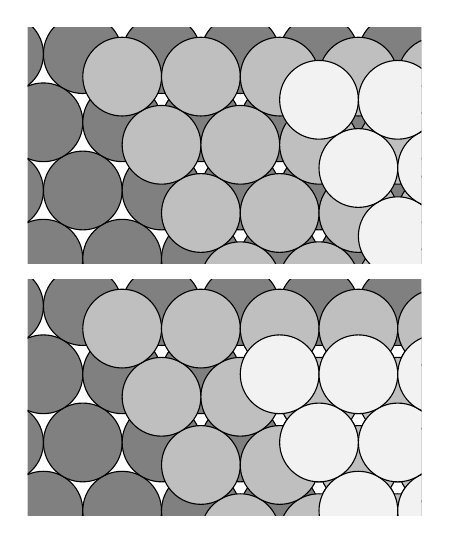
\begin{tikzpicture}

%\useasboundingbox (-1.3,-1.2) rectangle (11.2,4.7);
%	\draw (-1.5,-2.5) rectangle (3.5,7.5);


\begin{scope}[yshift=32mm]
  
 \clip (3mm,8mm) rectangle ++ (5cm, 3cm);  
   
 \foreach \u in {1,2,...,7}{%  
     \foreach \v in {1,2,...,4}{%  
            \draw[fill=gray] ({\u + \v * cos(120)}, {\v * sin(120) } )  circle (5mm) node (o\u\v) {};
         }
  }
  
   \foreach \u in {3,4,...,7}{%  
     \foreach \v in {1,2,...,4}{%  
            \draw[fill=gray!50!white] ({\u + \v * cos(120) + 0.5}, {(\v - 0.33) * sin(120) } )  circle (5mm) node (o\u\v) {};
         }
  }
  
  
   \foreach \u in {5,6,...,7}{%  
     \foreach \v in {1,2,...,3}{%  
            \draw[fill=gray!10!white] ({\u + \v * cos(120) + 0.5}, {(\v + 0.33) * sin(120) } )  circle (5mm) node (o\u\v) {};
         }
  }
\end{scope}

\begin{scope}
  
 \clip (3mm,8mm) rectangle ++ (5cm, 3cm);  
   
 \foreach \u in {1,2,...,7}{%  
     \foreach \v in {1,2,...,4}{%  
            \draw[fill=gray] ({\u + \v * cos(120)}, {\v * sin(120) } )  circle (5mm) node (o\u\v) {};
         }
  }
  
   \foreach \u in {3,4,...,7}{%  
     \foreach \v in {1,2,...,4}{%  
            \draw[fill=gray!50!white] ({\u + \v * cos(120) + 0.5}, {(\v - 0.33) * sin(120) } )  circle (5mm) node (o\u\v) {};
         }
  }
  
  
   \foreach \u in {5,6,...,7}{%  
     \foreach \v in {1,2,...,3}{%  
            \draw[fill=gray!10!white] ({\u + \v * cos(120) }, {(\v ) * sin(120) } )  circle (5mm) node (o\u\v) {};
         }
  }
\end{scope}
  
%  
%  \draw[thick, red,rotate around={30:(2.7,3.2) } ] (2.7,3.2) ellipse (7mm and 3mm);
%  \draw[thick, red] (1,1.7) ellipse (2mm and 5mm);
%
%  \node[below] at (u32) {\footnotesize P};  
%  \node[below] at (u42) {\footnotesize R};  
%  \node[above] at (o31) {\footnotesize Q};  
%  

     

  \end{tikzpicture}



